%----------------------------------------------------------------------------
\chapter{\bevezetes}
%----------------------------------------------------------------------------

A digitális eszközök térhódítása napjainkban az élet szinte minden területére kihat, és különösen nagy szerepet kaphatana az oktatásban is.
Mindig is fontosnak tartottam, hogy az oktatás teljes mértékben kihasználja a digitalizációban rejlő lehetőségeket, ezért esett a választásom erre a témára.

Úgy látom, hogy napjainkabn nincs eleggé kihasználva a technológiákban rejlő számtalan lehetőség az oktatás területén.
A családban erről több oldalról is kaptam visszajelzést.
Mivel nekem van lehetőségem informatikusként ezt a folyamatot segíteni és gyorsítani ezért kötelességemnek is tartom, hogy a digitalizáció integrálásával az oktatásba segítsem a legújabb generációkat.

A program, amelyet ebben a dolgozatban bemutatok, egy mobil- és egy asztali alkalmazás segítségével teszi lehetővé feladatsorok és dolgozatok előállítását PDF formátumban, nyomtatható változatban. Ebben a fejezetben kitérek arra, hogy miért döntöttem a Compose Multiplatform használata mellett, és ismertetem annak jelentőségét és elterjedtségét.
A fejezet végén rövid áttekintést nyújtok a dolgozat további szerkezeti elemeiről.

\section{Témaválasztás indoklása}

2023/2024 őszi félévében ismerkedtem meg a mobil, azon belül is az Android fejlesztéssel.
Az ezt követő félévben tovább mélyítettem a tudásomat ebben a témában, az Önálló laboratórium tárgy keretein belül elkezdtem fejleszteni a szakdolgozatom alapjaként szolgáló alkalmazást.
Szintén ebben a félévben hallgattam az Android alapú szoftverfejlesztés és a Kotlin alapú szoftverfejlesztés tárgyakat, amik segítettek jobban megérteni ezt a területet.
Az így elsajátított tudás és az önálló kutatás és tanulás során előállt egy Kotlin nyelven írt REST API, ami egy PostgreSQL adatbázissal biztosít kommunikációt, és természetesen egy Android alkalmazás, amelyet a szakdolgozat során tovább bővítettem és alakítottam át egy cross-platform szoftverré.

A kérdéssor összeállító alkalmazás ötletét a konzulensem vetette fel, hasznos lenne, ha létezne egy ilyen eszköz, amivel könnyen megoldható ez a feladat.
Megtetszett nekem is az ötlet, mivel vannak ismerőseim és családtagjaim, akik szintén tudnának egy ilyen alkalmazást hasznosítani a munkájuk vagy egyéb elfoglaltságaik kapcsán.
Egy nagyobb méretű fullstack alkalmazás előállítása túlmutat az Önálló laboratórium keretein, így rengeteg fejlesztési ötlet és lehetőség nem fért bele a félévbe.
Továbbgondolva ezt a projektet, folytattam a munkát a szoftveren.
Ezen kívül mindig szeretek új és érdekes dolgokat kipróbálni, és ha megtetszik, alaposan tanulmányozni és megtanulni.
Pont ezért választottam a Google és a JetBrains legújabb megoldásait a szakdolgozathoz.

A most elkészített szoftvert jelentősen tovább lehet még fejleszteni, felhasználók, szervezetek regisztrálásával és elkülönítésével, több fajta kérdéstípus megvalósításával.
Bevezetni a szervezeteken belül az oktató és diák csoportokat, és egy online kitöltési formát is megtervezni, létrehozni.
Az Önálló laboratórium alatt is élveztem ezzel foglalkozni, és még mindig szívesen fejleszteném tovább, és tenném jobbá az alkalmazást.

\section{Felhasznált technológia jelentősége/elterjedtsége}
\label{sec:IntroductionTechnologies}

Megfigyelve a mai trendeket, láttam, hogy a multiplatform fejlesztés egyre népszerűbb, mivel gyorsabban és hatékonyabban lehet egyszerűbb alkalmazásokat elkészíteni több fajta felhasználói réteg számára.
Úgy döntöttem, hogy kipróbálok egy új megoldást, ami a Compose Multiplatform; 2021 augusztusában jelent meg az 1.0 alpha verziója, és ezt a Kotlin Multiplatform egy évvel korábbi megjelenése tette lehetővé.
Az Android fejlesztők körében kifejezetten népszerű lett, annak ellenére is, hogy még mindig van rengeteg funkció, amit nem támogat, de jelenleg is aktívan fejlesztik, és válik hónapról-hónapra egyre jobbá.
A fejlesztések havonta / néhány havonta érkeznek mind a Kotlin nyelvhez és a Kotlin Multiplatformhoz\cite{KotlinMultiplatformRelease}, mind a Compose Multiplatformhoz\cite{ComposeMultiplatformRelease}.
Jelenleg vannak sokkal jobban elterjedt, használtabb cross-platform keretrendszerek, mint például a Flutter (\refstruc{fig:FlutterVsCompose}) vagy a React Native, ami iOS és Android fejlesztést tesz lehetővé JavaScript/TypeScript nyelven, így a webes fejlesztők gyakran használják natív mobilos appokhoz.

Szerencsére a fejlesztés folyamatos és gyors, amit segít az is, hogy sok nyílt forráskódú könyvtár is készül a felhasználók által.\cite{KotlinMultiplatformStable}
A Compose Multiplatform ennek az ellenpontja lesz\cite{KotlinCrossPlatformFrameworks}; sajnos a webes támogatás még csak alpha verzióban van, így eléggé instabil, és sok olyan eszköz nem használható még, ami a többi területen már stabilan működik, így ezzel egyelőre a szakdolgozat keretein belül nem foglalkoztam részletesebben a webes megoldás megvalósításával.

\begin{figure}[!ht]
    \centering
    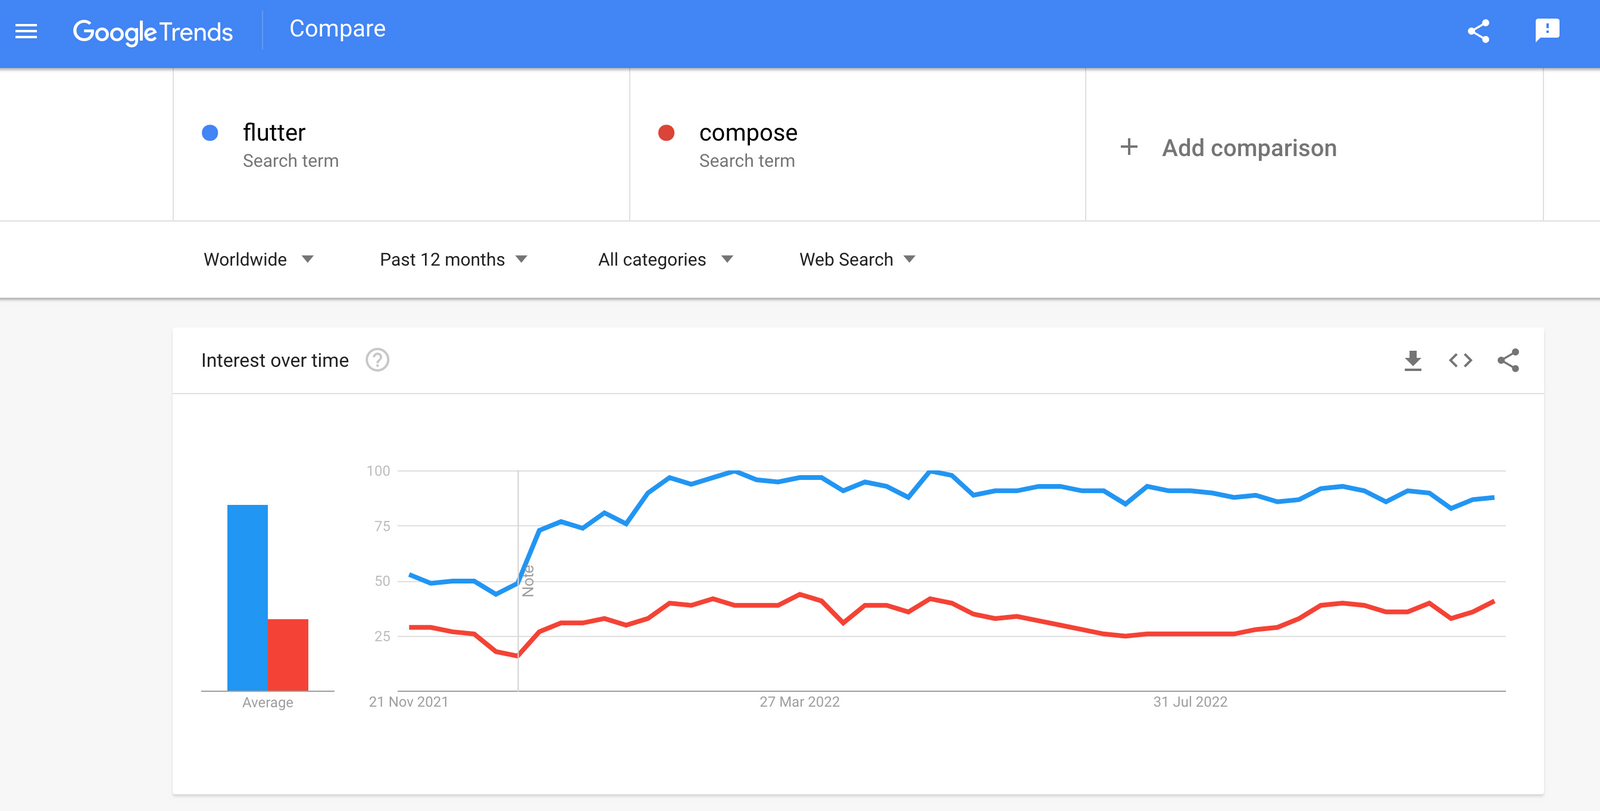
\includegraphics[width=150mm, keepaspectratio]{figures/flutter-vs-jetpack-compose-google-search-trends.png}
    \caption{A Flutter és a Compose keresési arányai \cite{FlutterVsCompose}}
    \label{fig:FlutterVsCompose}
\end{figure}

\begin{figure}[!ht]
    \centering
    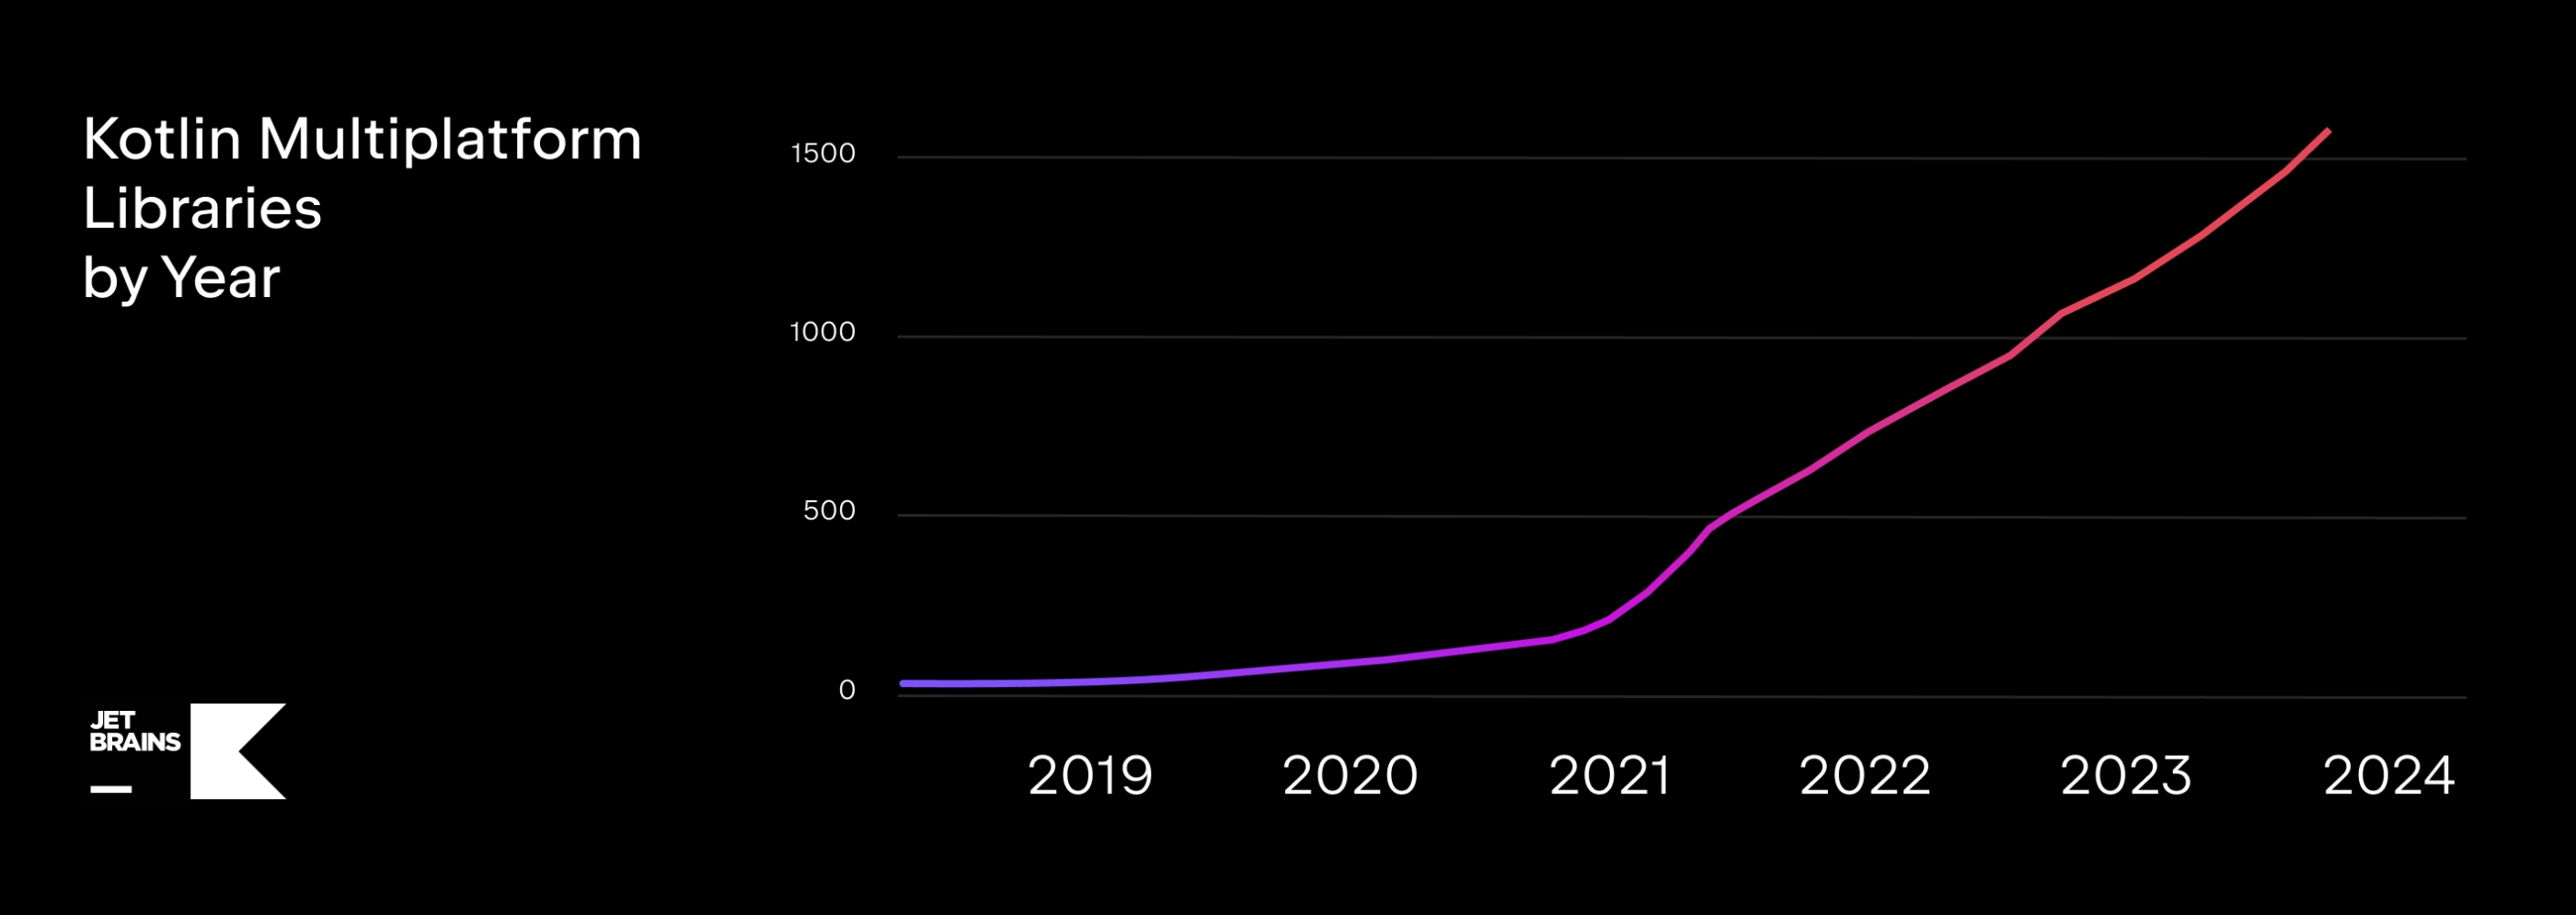
\includegraphics[width=150mm, keepaspectratio]{figures/Libraries-2800x995.png}
    \caption{A könyvtárak növekedésének gyors üteme \cite{KotlinMultiplatformStable}}
    \label{fig:KMPLibraries}
\end{figure}

A visszajelzések és a mostani szoftverfejlesztési irányokból arra lehet következtetni, hogy még hosszú jövő áll a technológiák előtt.
Könnyen, gyorsan és hatékonyan lehet akár egyszerre az összes platformra alkalmazást fejleszteni, nagy méretű közös és kis méretű natív kódbázis írásával és karbantartásával, összesen két nyelv ismeretével.
Webre, Androidra és asztali alkalmazáshoz elegendő lehet a Kotlin nyelv, esetleg egy kis HTML és JavaScript ismeret; iOS esetén minimális Swift és SwiftUI ismeret jól jöhet, de ez hasonlít a Kotlinra és a Compose-ra.
Az a tény, hogy a Compose Multiplatform csupán Kotlin nyelven írt kódbázissal képes natívan megjeleníteni az elkészült alkalmazást minden platformon, nagyon erős eszközzé teszi.
Például az Androidon futó alkalmazás az Androidos gombokat, görgetést stb. használja, míg iOS-en az ott megszokott stílust és irányítást kapja a felhasználó.

\section{Dolgozat felépítése}

A dolgozat felépítését az alábbi szerkezet szerint mutatom be. Az első fő rész a \textbf{feladatspecifikáció} (\refstruc{sec:Sepcification}), amelyben bemutatom a kitűzött feladatot, annak céljait és elvárásait. Ez a fejezet két alfejezetre oszlik: az elsőben részletesen ismertetem a feladatot (\refstruc{sec:SepcificationDescription}), míg a másodikban olyan diagramokat és ábrákat mutatok be (\refstruc{sec:SpecificationDiagrams}), amelyek segítik az alkalmazás felépítésének megértését.

Ezt követi az \textbf{irodalomkutatás} (\refstruc{sec:Search}), amely során részletezem az általam felhasznált technológiákat (\refstruc{sec:Technologies}), beleértve a \refstruc{sec:IntroductionTechnologies} szakaszban ismertetett könyvtárakat. Továbbá rövid összevetést készítek a hasonló cross-platform megoldásokkal (\refstruc{sec:SimilarSolutions}).

A harmadik fejezet a \textbf{felsőszintű architektúra} (\refstruc{sec:Architecture}), amelyben nagyvonalakban bemutatom az alkalmazás fő vázát és felépítését. Ez a rész két alfejezetből áll: az első a high-level architektúrával (\refstruc{sec:HighLevelArchitecture}), a második pedig a rendszer komponenseinek és azok kapcsolódásainak bemutatásával (\refstruc{sec:Components}) foglalkozik.

A dolgozat egyik központi része a \textbf{részletes megvalósítás} (\refstruc{sec:Details}), ahol minden korábban ismertetett technológia alkalmazását pontosan bemutatom, és részletezem, hogy ezek nálam milyen formában jelennek meg. Ennek a fejezetnek számos alfejezete van, amelyek a következő témákat fedik le: a Compose keretrendszer (\refstruc{sec:Compose}), a navigáció megvalósítása (\refstruc{sec:Nav}), a ViewModel használata (\refstruc{sec:VM}), az HTTP kliens implementációja (\refstruc{sec:HTTP}), a PDF-kezelés (\refstruc{sec:PDF}), valamint a szövegfelismerési funkciók (\refstruc{sec:TextRec}).

A dolgozat utolsó előtti fejezete a \textbf{továbbfejlesztési lehetőségek} (\refstruc{sec:Future}), amelyben áttekintem, milyen irányokba fejleszthető tovább az alkalmazás. Végül az összefoglalás (\refstruc{sec:Summary}) fejezetben összegzem a dolgozat legfontosabb eredményeit és megfogalmazom a levont tanulságokat.
